\documentclass[a4paper, landscape, 12pt]{article}

\usepackage[left = 2cm, bottom = 3cm, right = 3cm, top = 2cm]{geometry}
\usepackage{pgfplots}

\pagestyle{empty}

\begin{document}
\begin{figure}
    \centering
    \large

    \textit{Laufzeitmessungen und Werte der Formel für $M = 3$ und $1 \le k_i \le 6$}
    \vspace{1.5em}

    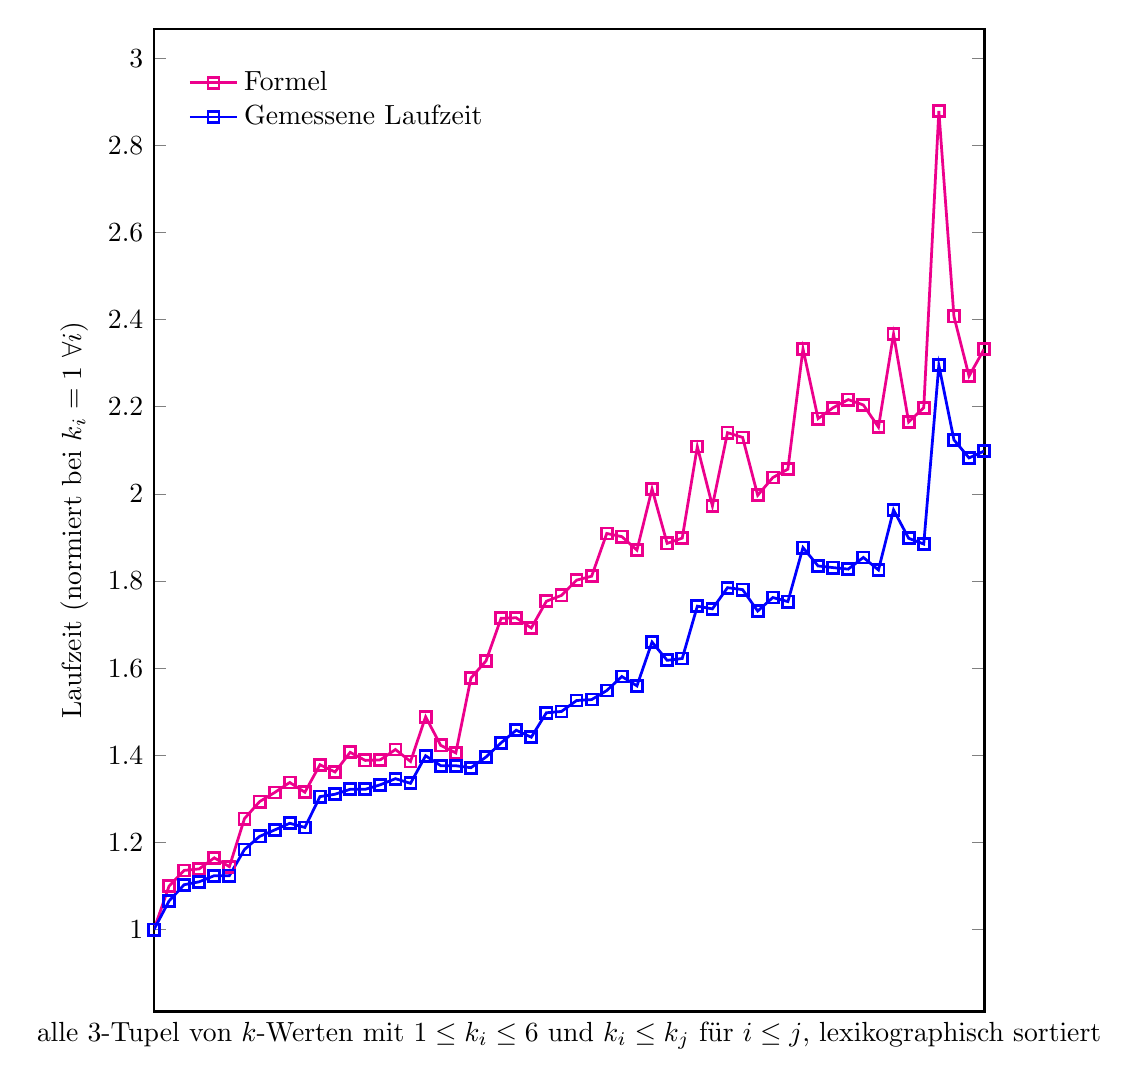
\begin{tikzpicture}
        \begin{axis}[
                xlabel = {alle 3-Tupel von $k$-Werten mit $1 \le k_i \le 6$ und $k_i \le k_j$ für $i \le j$, lexikographisch sortiert},
                ylabel = {Laufzeit (normiert bei $k_i = 1 \ \forall i$)},
                xmin = 1,
                xmax = 56,
                xmajorticks=false,
                width = \textwidth,
                height = 400pt,
                legend pos = north west,
                legend style = {draw = none},
                legend cell align = left,
                line width = 1pt,
            ]

            \addplot[color = magenta, mark = square]
            coordinates {
                    (1, 1)
                    (2, 1.0995832370567191)
                    (3, 1.1358269318848557)
                    (4, 1.1393205365715215)
                    (5, 1.1647721717331307)
                    (6, 1.144442289069)
                    (7, 1.2548293386917135)
                    (8, 1.293751480016151)
                    (9, 1.314659878659051)
                    (10, 1.33768582148081)
                    (11, 1.3152982280215748)
                    (12, 1.3784086819046726)
                    (13, 1.3617280369815357)
                    (14, 1.4069269490894507)
                    (15, 1.388384818389762)
                    (16, 1.3896278178685892)
                    (17, 1.4133641301874809)
                    (18, 1.3858584388316284)
                    (19, 1.488476182385774)
                    (20, 1.422868622651227)
                    (21, 1.4055588897855955)
                    (22, 1.5773502691896257)
                    (23, 1.616719569871336)
                    (24, 1.714534014225912)
                    (25, 1.7156703208960307)
                    (26, 1.6922850974516965)
                    (27, 1.753639955129007)
                    (28, 1.767104822278083)
                    (29, 1.802049224794656)
                    (30, 1.8111605132977815)
                    (31, 1.909231425915723)
                    (32, 1.901925232568137)
                    (33, 1.870984269392369)
                    (34, 2.0114963891668403)
                    (35, 1.8864202722907604)
                    (36, 1.8985991908695523)
                    (37, 2.1086517918741277)
                    (38, 1.9723786016023641)
                    (39, 2.140613031123653)
                    (40, 2.129605365022787)
                    (41, 1.9967960595532597)
                    (42, 2.0375215568106513)
                    (43, 2.0567917282158037)
                    (44, 2.3328768129943143)
                    (45, 2.1727988105183047)
                    (46, 2.1979636724393874)
                    (47, 2.21648605664914)
                    (48, 2.2041388623134517)
                    (49, 2.153288505654449)
                    (50, 2.366810016830746)
                    (51, 2.1650994932357537)
                    (52, 2.1979077179237216)
                    (53, 2.8790043489023804)
                    (54, 2.407453281490819)
                    (55, 2.270382394967579)
                    (56, 2.332272327437964)
                };

            \addplot[color = blue, mark = square]
            coordinates{
                    (1, 1)
                    (2, 1.065584516150987)
                    (3, 1.1029946191769353)
                    (4, 1.1097933054183466)
                    (5, 1.123811640427135)
                    (6, 1.1238892496304664)
                    (7, 1.1838623942943398)
                    (8, 1.213932805227455)
                    (9, 1.2287818090789364)
                    (10, 1.244075407998243)
                    (11, 1.23450475997349)
                    (12, 1.305249542542411)
                    (13, 1.3106957061380258)
                    (14, 1.3220861034082012)
                    (15, 1.3219863070573987)
                    (16, 1.3324499682974158)
                    (17, 1.3464258164993392)
                    (18, 1.3357442076524222)
                    (19, 1.3990501454477926)
                    (20, 1.3762731052678283)
                    (21, 1.3761335044506202)
                    (22, 1.3715394890371406)
                    (23, 1.3960860744865695)
                    (24, 1.4287401336170678)
                    (25, 1.457689051361297)
                    (26, 1.441602799075183)
                    (27, 1.4977047469241669)
                    (28, 1.500669454683552)
                    (29, 1.5257853468523568)
                    (30, 1.527959581935043)
                    (31, 1.5486799037808971)
                    (32, 1.580883561068963)
                    (33, 1.5594554976227282)
                    (34, 1.660032640853586)
                    (35, 1.6180969324037537)
                    (36, 1.6222763441103245)
                    (37, 1.7423713326808168)
                    (38, 1.7361480508447782)
                    (39, 1.7847888751471053)
                    (40, 1.7802892433000512)
                    (41, 1.7311530152247514)
                    (42, 1.762179528203984)
                    (43, 1.752867202622113)
                    (44, 1.8768094233227084)
                    (45, 1.83462867127512)
                    (46, 1.8308478677302598)
                    (47, 1.827375895259475)
                    (48, 1.8541801340601693)
                    (49, 1.8253585484606458)
                    (50, 1.963258963393976)
                    (51, 1.8981154849455428)
                    (52, 1.8849166610677677)
                    (53, 2.295177938231215)
                    (54, 2.1240353558677465)
                    (55, 2.082654898764909)
                    (56, 2.0981695147498822)
                };

            \legend{Formel, Gemessene Laufzeit}
        \end{axis}
    \end{tikzpicture}



\end{figure}
\end{document}